\subsection{Development methodology of mechatronics --- VDI 2206}
\label{subsec:vdi-2206}

Mechatronics, was defined by Harashima et. al~\cite{harashima1996mechatronics}
as: \emph{''the synergistic integration of mechanical engineering
with electronic and intelligent computer control in the design of industrial
products and processes''}. This definition has more than twenty years, and
nowadays it could be extended to other domains beyond the industrial sector,
but a central idea remains: the synergy between these fields of knowledge, able
% src:
% https://en.wikibooks.org/wiki/LaTeX/Floats,_Figures_and_Captions#Subfloats
\begin{figure}[!hbt]
    \centering
    %\captionsetup[sub]{margin=10pt}
    % a)
    \subcaptionbox{One macro cycle
\label{fig:v-model-macro}}
    [0.5\linewidth]{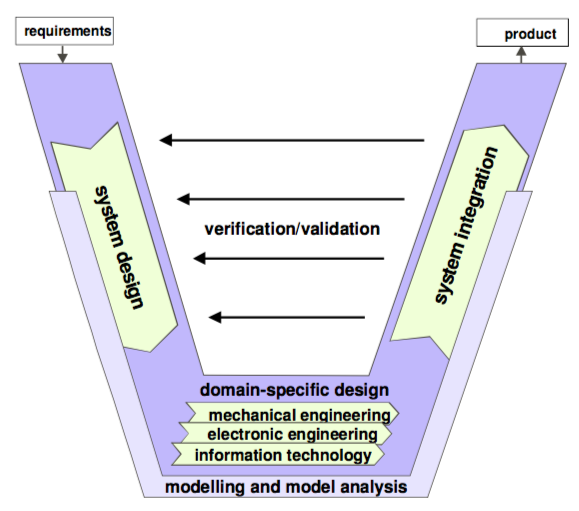
\includegraphics[width=0.45\textwidth]{./img/v-model-macro.png}}
    % b)
    %\subcaptionbox{One macro cycle (refined)~\cite{isermann2008mechatronic} 
    %\label{fig:v-model-isermann}}
    %[0.8\linewidth]{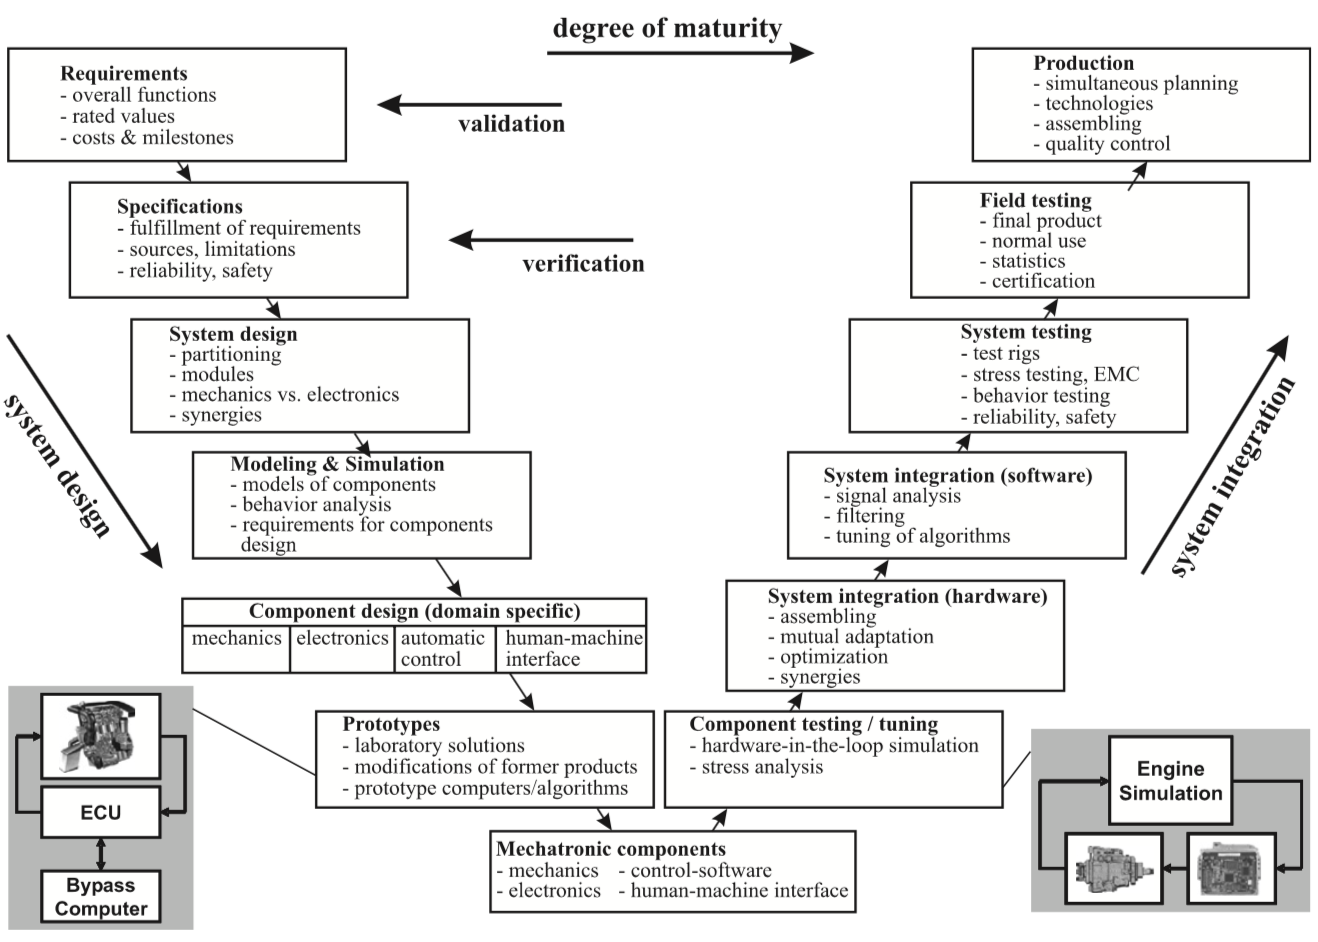
\includegraphics[width=0.8\textwidth]{./img/v-model-isermann.png}}
    % b)
    \subcaptionbox{Iterating over a number of macro-cycles with increasing
      process maturity
\label{fig:v-model-iter}}
    [1.0\linewidth]{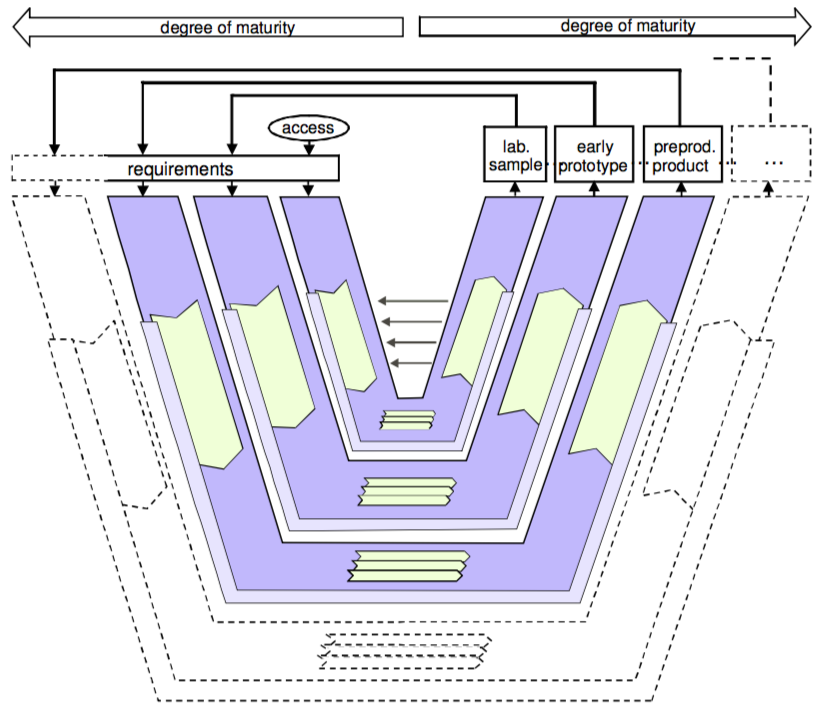
\includegraphics[width=0.55\textwidth]{./img/v-model-iter.png}}
    % c)
    % fig
    \caption{Mechatronics design V-model, VDI 2206 2003~\cite{gausemeier2003new}}
\label{fig:v-model}
\end{figure}

\subsubsection{Process modules for recurrent working steps}
The main phases in the v-model are not yet detailed: this needs to be done by
the designer. However, some design procedures occur regularly during the design
and were identified by field practitioners in terms of predefined process
modules, representing procedures and methods for different design tasks,
organised in a data base
(fig.~\ref{fig:v-model-recurrent}\cite{gausemeier2003new}). The VDI 2206
guideline provides detailed process modules for the V-model macro cycle. One
such example is given in fig.~\ref{fig:v-model-recurrent} for the system design,
which can be described phase-milestone-diagrams, checklists, process-flow
diagrams, etc..

\begin{figure}[!hbt]
  \begin{center}
    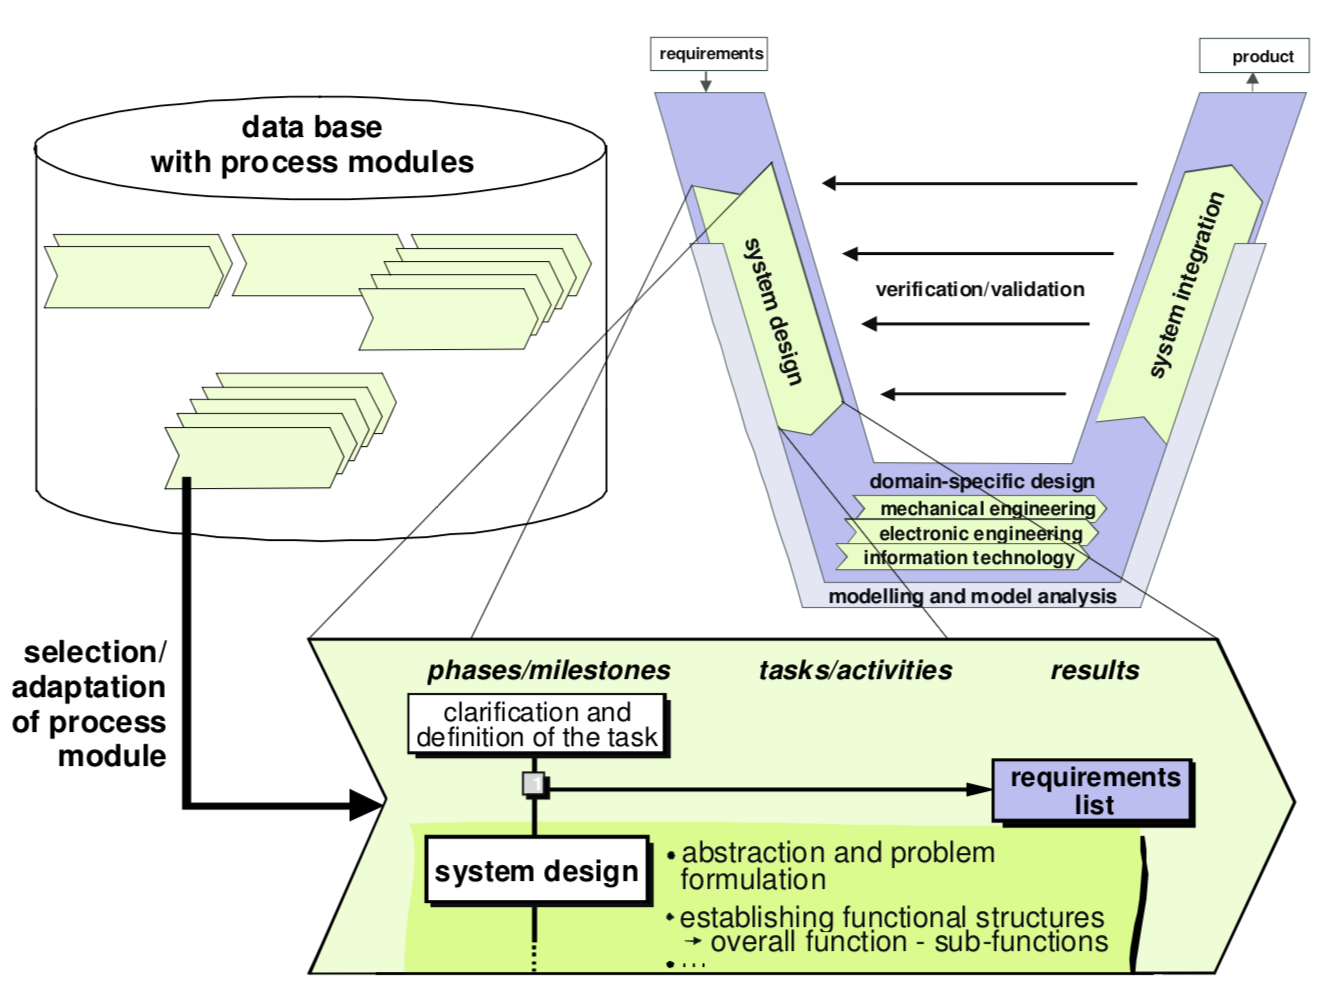
\includegraphics[width=0.65\textwidth]{./img/v-model-recurrent.png}
  \end{center}
  \caption{Configuration of process modules for individual operation steps}
\label{fig:v-model-recurrent}
\end{figure}

%%% Local Variables:
%%% mode: latex
%%% TeX-master: "../../../dissertation"
%%% End:
